%% bare_conf.tex
%% V1.3
%% 2007/01/11
%% by Michael Shell
%% See:
%% http://www.michaelshell.org/
%% for current contact information.
%%
%% This is a skeleton file demonstrating the use of IEEEtran.cls
%% (requires IEEEtran.cls version 1.7 or later) with an IEEE conference paper.
%%
%% Support sites:
%% http://www.michaelshell.org/tex/ieeetran/
%% http://www.ctan.org/tex-archive/macros/latex/contrib/IEEEtran/
%% and
%% http://www.ieee.org/

%%*************************************************************************
%% Legal Notice:
%% This code is offered as-is without any warranty either expressed or
%% implied; without even the implied warranty of MERCHANTABILITY or
%% FITNESS FOR A PARTICULAR PURPOSE!
%% User assumes all risk.
%% In no event shall IEEE or any contributor to this code be liable for
%% any damages or losses, including, but not limited to, incidental,
%% consequential, or any other damages, resulting from the use or misuse
%% of any information contained here.
%%
%% All comments are the opinions of their respective authors and are not
%% necessarily endorsed by the IEEE.
%%
%% This work is distributed under the LaTeX Project Public License (LPPL)
%% ( http://www.latex-project.org/ ) version 1.3, and may be freely used,
%% distributed and modified. A copy of the LPPL, version 1.3, is included
%% in the base LaTeX documentation of all distributions of LaTeX released
%% 2003/12/01 or later.
%% Retain all contribution notices and credits.
%% ** Modified files should be clearly indicated as such, including  **
%% ** renaming them and changing author support contact information. **
%%
%% File list of work: IEEEtran.cls, IEEEtran_HOWTO.pdf, bare_adv.tex,
%%                    bare_conf.tex, bare_jrnl.tex, bare_jrnl_compsoc.tex
%%*************************************************************************

% *** Authors should verify (and, if needed, correct) their LaTeX system  ***
% *** with the testflow diagnostic prior to trusting their LaTeX platform ***
% *** with production work. IEEE's font choices can trigger bugs that do  ***
% *** not appear when using other class files.                            ***
% The testflow support page is at:
% http://www.michaelshell.org/tex/testflow/



% Note that the a4paper option is mainly intended so that authors in
% countries using A4 can easily print to A4 and see how their papers will
% look in print - the typesetting of the document will not typically be
% affected with changes in paper size (but the bottom and side margins will).
% Use the testflow package mentioned above to verify correct handling of
% both paper sizes by the user's LaTeX system.
%
% Also note that the "draftcls" or "draftclsnofoot", not "draft", option
% should be used if it is desired that the figures are to be displayed in
% draft mode.
%\documentclass[10pt, conference, compsocconf]{IEEEtran}%
% CHANGE TO 9 pt for the long abstract
\documentclass[9pt, conference, compsocconf]{IEEEtran}

% Add the compsocconf option for Computer Society conferences.
%
% If IEEEtran.cls has not been installed into the LaTeX system files,
% manually specify the path to it like:
% \documentclass[conference]{../sty/IEEEtran}




% Some very useful LaTeX packages include:
% (uncomment the ones you want to load)


% *** MISC UTILITY PACKAGES ***
%
%\usepackage{ifpdf}
% Heiko Oberdiek's ifpdf.sty is very useful if you need conditional
% compilation based on whether the output is pdf or dvi.
% usage:
% \ifpdf
%   % pdf code
% \else
%   % dvi code
% \fi
% The latest version of ifpdf.sty can be obtained from:
% http://www.ctan.org/tex-archive/macros/latex/contrib/oberdiek/
% Also, note that IEEEtran.cls V1.7 and later provides a builtin
% \ifCLASSINFOpdf conditional that works the same way.
% When switching from latex to pdflatex and vice-versa, the compiler may
% have to be run twice to clear warning/error messages.






% *** CITATION PACKAGES ***
%
%\usepackage{cite}
% cite.sty was written by Donald Arseneau
% V1.6 and later of IEEEtran pre-defines the format of the cite.sty package
% \cite{} output to follow that of IEEE. Loading the cite package will
% result in citation numbers being automatically sorted and properly
% "compressed/ranged". e.g., [1], [9], [2], [7], [5], [6] without using
% cite.sty will become [1], [2], [5]--[7], [9] using cite.sty. cite.sty's
% \cite will automatically add leading space, if needed. Use cite.sty's
% noadjust option (cite.sty V3.8 and later) if you want to turn this off.
% cite.sty is already installed on most LaTeX systems. Be sure and use
% version 4.0 (2003-05-27) and later if using hyperref.sty. cite.sty does
% not currently provide for hyperlinked citations.
% The latest version can be obtained at:
% http://www.ctan.org/tex-archive/macros/latex/contrib/cite/
% The documentation is contained in the cite.sty file itself.






% *** GRAPHICS RELATED PACKAGES ***
%
\ifCLASSINFOpdf
  % \usepackage[pdftex]{graphicx}
  % declare the path(s) where your graphic files are
  % \graphicspath{{../pdf/}{../jpeg/}}
  % and their extensions so you won't have to specify these with
  % every instance of \includegraphics
  % \DeclareGraphicsExtensions{.pdf,.jpeg,.png}
\else
  % or other class option (dvipsone, dvipdf, if not using dvips). graphicx
  % will default to the driver specified in the system graphics.cfg if no
  % driver is specified.
  % \usepackage[dvips]{graphicx}
  % declare the path(s) where your graphic files are
  % \graphicspath{{../eps/}}
  % and their extensions so you won't have to specify these with
  % every instance of \includegraphics
  % \DeclareGraphicsExtensions{.eps}
\fi
% graphicx was written by David Carlisle and Sebastian Rahtz. It is
% required if you want graphics, photos, etc. graphicx.sty is already
% installed on most LaTeX systems. The latest version and documentation can
% be obtained at:
% http://www.ctan.org/tex-archive/macros/latex/required/graphics/
% Another good source of documentation is "Using Imported Graphics in
% LaTeX2e" by Keith Reckdahl which can be found as epslatex.ps or
% epslatex.pdf at: http://www.ctan.org/tex-archive/info/
%
% latex, and pdflatex in dvi mode, support graphics in encapsulated
% postscript (.eps) format. pdflatex in pdf mode supports graphics
% in .pdf, .jpeg, .png and .mps (metapost) formats. Users should ensure
% that all non-photo figures use a vector format (.eps, .pdf, .mps) and
% not a bitmapped formats (.jpeg, .png). IEEE frowns on bitmapped formats
% which can result in "jaggedy"/blurry rendering of lines and letters as
% well as large increases in file sizes.
%
% You can find documentation about the pdfTeX application at:
% http://www.tug.org/applications/pdftex





% *** MATH PACKAGES ***
%
%\usepackage[cmex10]{amsmath}
% A popular package from the American Mathematical Society that provides
% many useful and powerful commands for dealing with mathematics. If using
% it, be sure to load this package with the cmex10 option to ensure that
% only type 1 fonts will utilized at all point sizes. Without this option,
% it is possible that some math symbols, particularly those within
% footnotes, will be rendered in bitmap form which will result in a
% document that can not be IEEE Xplore compliant!
%
% Also, note that the amsmath package sets \interdisplaylinepenalty to 10000
% thus preventing page breaks from occurring within multiline equations. Use:
%\interdisplaylinepenalty=2500
% after loading amsmath to restore such page breaks as IEEEtran.cls normally
% does. amsmath.sty is already installed on most LaTeX systems. The latest
% version and documentation can be obtained at:
% http://www.ctan.org/tex-archive/macros/latex/required/amslatex/math/





% *** SPECIALIZED LIST PACKAGES ***
%
%\usepackage{algorithmic}
% algorithmic.sty was written by Peter Williams and Rogerio Brito.
% This package provides an algorithmic environment fo describing algorithms.
% You can use the algorithmic environment in-text or within a figure
% environment to provide for a floating algorithm. Do NOT use the algorithm
% floating environment provided by algorithm.sty (by the same authors) or
% algorithm2e.sty (by Christophe Fiorio) as IEEE does not use dedicated
% algorithm float types and packages that provide these will not provide
% correct IEEE style captions. The latest version and documentation of
% algorithmic.sty can be obtained at:
% http://www.ctan.org/tex-archive/macros/latex/contrib/algorithms/
% There is also a support site at:
% http://algorithms.berlios.de/index.html
% Also of interest may be the (relatively newer and more customizable)
% algorithmicx.sty package by Szasz Janos:
% http://www.ctan.org/tex-archive/macros/latex/contrib/algorithmicx/




% *** ALIGNMENT PACKAGES ***
%
%\usepackage{array}
% Frank Mittelbach's and David Carlisle's array.sty patches and improves
% the standard LaTeX2e array and tabular environments to provide better
% appearance and additional user controls. As the default LaTeX2e table
% generation code is lacking to the point of almost being broken with
% respect to the quality of the end results, all users are strongly
% advised to use an enhanced (at the very least that provided by array.sty)
% set of table tools. array.sty is already installed on most systems. The
% latest version and documentation can be obtained at:
% http://www.ctan.org/tex-archive/macros/latex/required/tools/


%\usepackage{mdwmath}
%\usepackage{mdwtab}
% Also highly recommended is Mark Wooding's extremely powerful MDW tools,
% especially mdwmath.sty and mdwtab.sty which are used to format equations
% and tables, respectively. The MDWtools set is already installed on most
% LaTeX systems. The lastest version and documentation is available at:
% http://www.ctan.org/tex-archive/macros/latex/contrib/mdwtools/


% IEEEtran contains the IEEEeqnarray family of commands that can be used to
% generate multiline equations as well as matrices, tables, etc., of high
% quality.


%\usepackage{eqparbox}
% Also of notable interest is Scott Pakin's eqparbox package for creating
% (automatically sized) equal width boxes - aka "natural width parboxes".
% Available at:
% http://www.ctan.org/tex-archive/macros/latex/contrib/eqparbox/





% *** SUBFIGURE PACKAGES ***
%\usepackage[tight,footnotesize]{subfigure}
% subfigure.sty was written by Steven Douglas Cochran. This package makes it
% easy to put subfigures in your figures. e.g., "Figure 1a and 1b". For IEEE
% work, it is a good idea to load it with the tight package option to reduce
% the amount of white space around the subfigures. subfigure.sty is already
% installed on most LaTeX systems. The latest version and documentation can
% be obtained at:
% http://www.ctan.org/tex-archive/obsolete/macros/latex/contrib/subfigure/
% subfigure.sty has been superceeded by subfig.sty.



%\usepackage[caption=false]{caption}
%\usepackage[font=footnotesize]{subfig}
% subfig.sty, also written by Steven Douglas Cochran, is the modern
% replacement for subfigure.sty. However, subfig.sty requires and
% automatically loads Axel Sommerfeldt's caption.sty which will override
% IEEEtran.cls handling of captions and this will result in nonIEEE style
% figure/table captions. To prevent this problem, be sure and preload
% caption.sty with its "caption=false" package option. This is will preserve
% IEEEtran.cls handing of captions. Version 1.3 (2005/06/28) and later
% (recommended due to many improvements over 1.2) of subfig.sty supports
% the caption=false option directly:
%\usepackage[caption=false,font=footnotesize]{subfig}
%
% The latest version and documentation can be obtained at:
% http://www.ctan.org/tex-archive/macros/latex/contrib/subfig/
% The latest version and documentation of caption.sty can be obtained at:
% http://www.ctan.org/tex-archive/macros/latex/contrib/caption/




% *** FLOAT PACKAGES ***
%
%\usepackage{fixltx2e}
% fixltx2e, the successor to the earlier fix2col.sty, was written by
% Frank Mittelbach and David Carlisle. This package corrects a few problems
% in the LaTeX2e kernel, the most notable of which is that in current
% LaTeX2e releases, the ordering of single and double column floats is not
% guaranteed to be preserved. Thus, an unpatched LaTeX2e can allow a
% single column figure to be placed prior to an earlier double column
% figure. The latest version and documentation can be found at:
% http://www.ctan.org/tex-archive/macros/latex/base/



%\usepackage{stfloats}
% stfloats.sty was written by Sigitas Tolusis. This package gives LaTeX2e
% the ability to do double column floats at the bottom of the page as well
% as the top. (e.g., "\begin{figure*}[!b]" is not normally possible in
% LaTeX2e). It also provides a command:
%\fnbelowfloat
% to enable the placement of footnotes below bottom floats (the standard
% LaTeX2e kernel puts them above bottom floats). This is an invasive package
% which rewrites many portions of the LaTeX2e float routines. It may not work
% with other packages that modify the LaTeX2e float routines. The latest
% version and documentation can be obtained at:
% http://www.ctan.org/tex-archive/macros/latex/contrib/sttools/
% Documentation is contained in the stfloats.sty comments as well as in the
% presfull.pdf file. Do not use the stfloats baselinefloat ability as IEEE
% does not allow \baselineskip to stretch. Authors submitting work to the
% IEEE should note that IEEE rarely uses double column equations and
% that authors should try to avoid such use. Do not be tempted to use the
% cuted.sty or midfloat.sty packages (also by Sigitas Tolusis) as IEEE does
% not format its papers in such ways.





% *** PDF, URL AND HYPERLINK PACKAGES ***
%
%\usepackage{url}
% url.sty was written by Donald Arseneau. It provides better support for
% handling and breaking URLs. url.sty is already installed on most LaTeX
% systems. The latest version can be obtained at:
% http://www.ctan.org/tex-archive/macros/latex/contrib/misc/
% Read the url.sty source comments for usage information. Basically,
% \url{my_url_here}.





% *** Do not adjust lengths that control margins, column widths, etc. ***
% *** Do not use packages that alter fonts (such as pslatex).         ***
% There should be no need to do such things with IEEEtran.cls V1.6 and later.
% (Unless specifically asked to do so by the journal or conference you plan
% to submit to, of course. )


% correct bad hyphenation here
%\hyphenation{op-tical net-works semi-conduc-tor}



%%%% ADD ADDITIONAL USEPACKAGE HERE %%%%%
\usepackage[pdftex]{graphicx}
\DeclareGraphicsExtensions{.pdf,.jpeg,.png}

\usepackage[cmex10]{amsmath}

% ACG added
\usepackage{tabulary}
%\usepackage{tabularx}

% ACG added for equation support
\usepackage{amsmath}

% ACG
%\usepackage[breaklinks]{hyperref}

% ACG added fmtcount for superscript support, e.g., \ordinalnum{18} = 18^th
\usepackage{fmtcount}

% ACG added hhline for double line support
\usepackage{hhline}

% ACG added for sweet tildes
\newcommand{\mytilde}{\raise.17ex\hbox{$\scriptstyle\mathtt{\sim}$}}

% ACG added for special chars in verbatim
\usepackage{alltt}

% ACG added for float figures
\usepackage{fixltx2e}

%ACG added for color comments
\usepackage{xcolor}
\newcommand{\comment}[1]
{\par {\bfseries \color{blue} #1 \par}} %comment showed

%ACG added for RED
\usepackage{xcolor}
\newcommand{\RED}[1]
{{\bfseries \color{red} #1}}

\usepackage{url}

%SJL added:
\usepackage{flushend}

\begin{document}

%
% paper title
% can use linebreaks \\ within to get better formatting as desired
\title{Supporting failure analysis with discoverable, annotated log datasets -- LONG ABSTRACT}
\author{Stephen Leak, Annette Greiner, Jim Brandt, and Ann Gentile}
%\author{\IEEEauthorblockN{Stephen Leak, Annette Greiner}
%\IEEEauthorblockA{National Energy Research Supercomputing Center (NERSC)\\
%Berkeley, CA, USA\\
%sleak@lbl.gov}
%\and
%\IEEEauthorblockN{James Brandt, Ann Gentile}
%\IEEEauthorblockA{Sandia National Laboratory (SNL)\\
%Albuquerque, NM and Livermore, CA, USA\\
%gentile@sandia.gov}
%}


% author names and affiliations
% use a multiple column layout for up to two different
% affiliations

%\author{\IEEEauthorblockN{Authors Name/s per 1st Affiliation (Author)}
%\IEEEauthorblockA{line 1 (of Affiliation): dept. name of organization\\
%line 2: name of organization, acronyms acceptable\\
%line 3: City, Country\\
%line 4: Email: name@xyz.com}
%\and
%\IEEEauthorblockN{Authors Name/s per 2nd Affiliation (Author)}
%\IEEEauthorblockA{line 1 (of Affiliation): dept. name of organization\\
%line 2: name of organization, acronyms acceptable\\
%line 3: City, Country\\
%line 4: Email: name@xyz.com}
%}

% conference papers do not typically use \thanks and this command
% is locked out in conference mode. If really needed, such as for
% the acknowledgment of grants, issue a \IEEEoverridecommandlockouts
% after \documentclass

% for over three affiliations, or if they all won't fit within the width
% of the page, use this alternative format:
%


% use for special paper notices
%\IEEEspecialpapernotice{(Invited Paper)}




% make the title area
\maketitle

\begin{abstract}
Detection, characterization, and mitigation of faults on supercomputers is
complicated by the large variety of interacting subsystems. Failures often
manifest as vague observations like ``my job failed" and may result from
faults in system
hardware/firmware/software, filesystems, networks, resource manager state, and
more.  Data such as system logs, environmental metrics, job history, cluster
state snapshots, published outage notices and user reports is routinely
collected. These data are typically stored in different locations and formats
for specific use by targeted consumers. Combining data sources for analysis
generally requires a consumer-dependent custom approach.  We present a
vocabulary for describing data, including format and access details, an
annotation schema for attaching observations to a dataset, and tools to aid in
discovery and publication of system-related insights. We present case studies in
which our analysis tools utilize information from disparate data sources to
investigate failures and performance issues from user and administrator perspectives.


\end{abstract}

% For peer review papers, you can put extra information on the cover
% page as needed:
% \ifCLASSOPTIONpeerreview
% \begin{center} \bfseries EDICS Category: 3-BBND \end{center}
% \fi
%
% For peerreview papers, this IEEEtran command inserts a page break and
% creates the second title. It will be ignored for other modes.
\IEEEpeerreviewmaketitle

\section{Context}
NERSC's Cori system has 2388 Xeon nodes, 9688 Xeon Phi nodes, a host of service nodes
providing I/O forwarding, a burst-buffer filesystem, Lustre networking and
system management, and an Aries high-speed network in a Dragonfly topology. Cori
has a large external Lustre filesystem also cross-mounted on Edison - another
large Cray system at NERSC - via Infiniband. It has external login nodes and shares
GPFS filesystems with other NERSC servers. There are air and water cooling
components and UPS power circuits. Along with Cray system software
and programming environments, Cori runs multiple compilers and MPI stacks and
hundreds of software packages. Its 7,000 users run tens of thousands of jobs per
day via the Slurm batch scheduler.

At this scale and complexity the identification and characterization of faults
leading to failures is both important and difficult. Important because for
reliability at scale we must identify the points in the system whose failure is
most impactful; difficult because of the variety of sources and formats of log
data to consider when investigating failures.
This challenge has been identified by other Cray sites and there are efforts within
the Cray community to improve our ability to detect, characterize and mitigate
faults in this complex environment.

Data such as system logs, environmental metrics, job history, filesystem state,
outage notices and user reports are already routinely collected. There are
multiple domains within the ecosystem of an HPC center which are typically
tended by different teams. Details of data collection and storage typically
target the associated team's specific needs. Discovering, accessing and
combining information from these disparate data
sources for a failure investigation can be difficult and time-consuming.

System-generated logs identify faults but not the context in which they
occurred or whether they actually resulted in failure. ``Failure" is often
vaguely defined, such as a job seeing a significant performance reduction on a
specific occasion. Overlaying logs with human-made observations adds clarifying
information about the context and outcome of events, but these observations may
be imprecise or inaccurate.

\begin{figure*}
  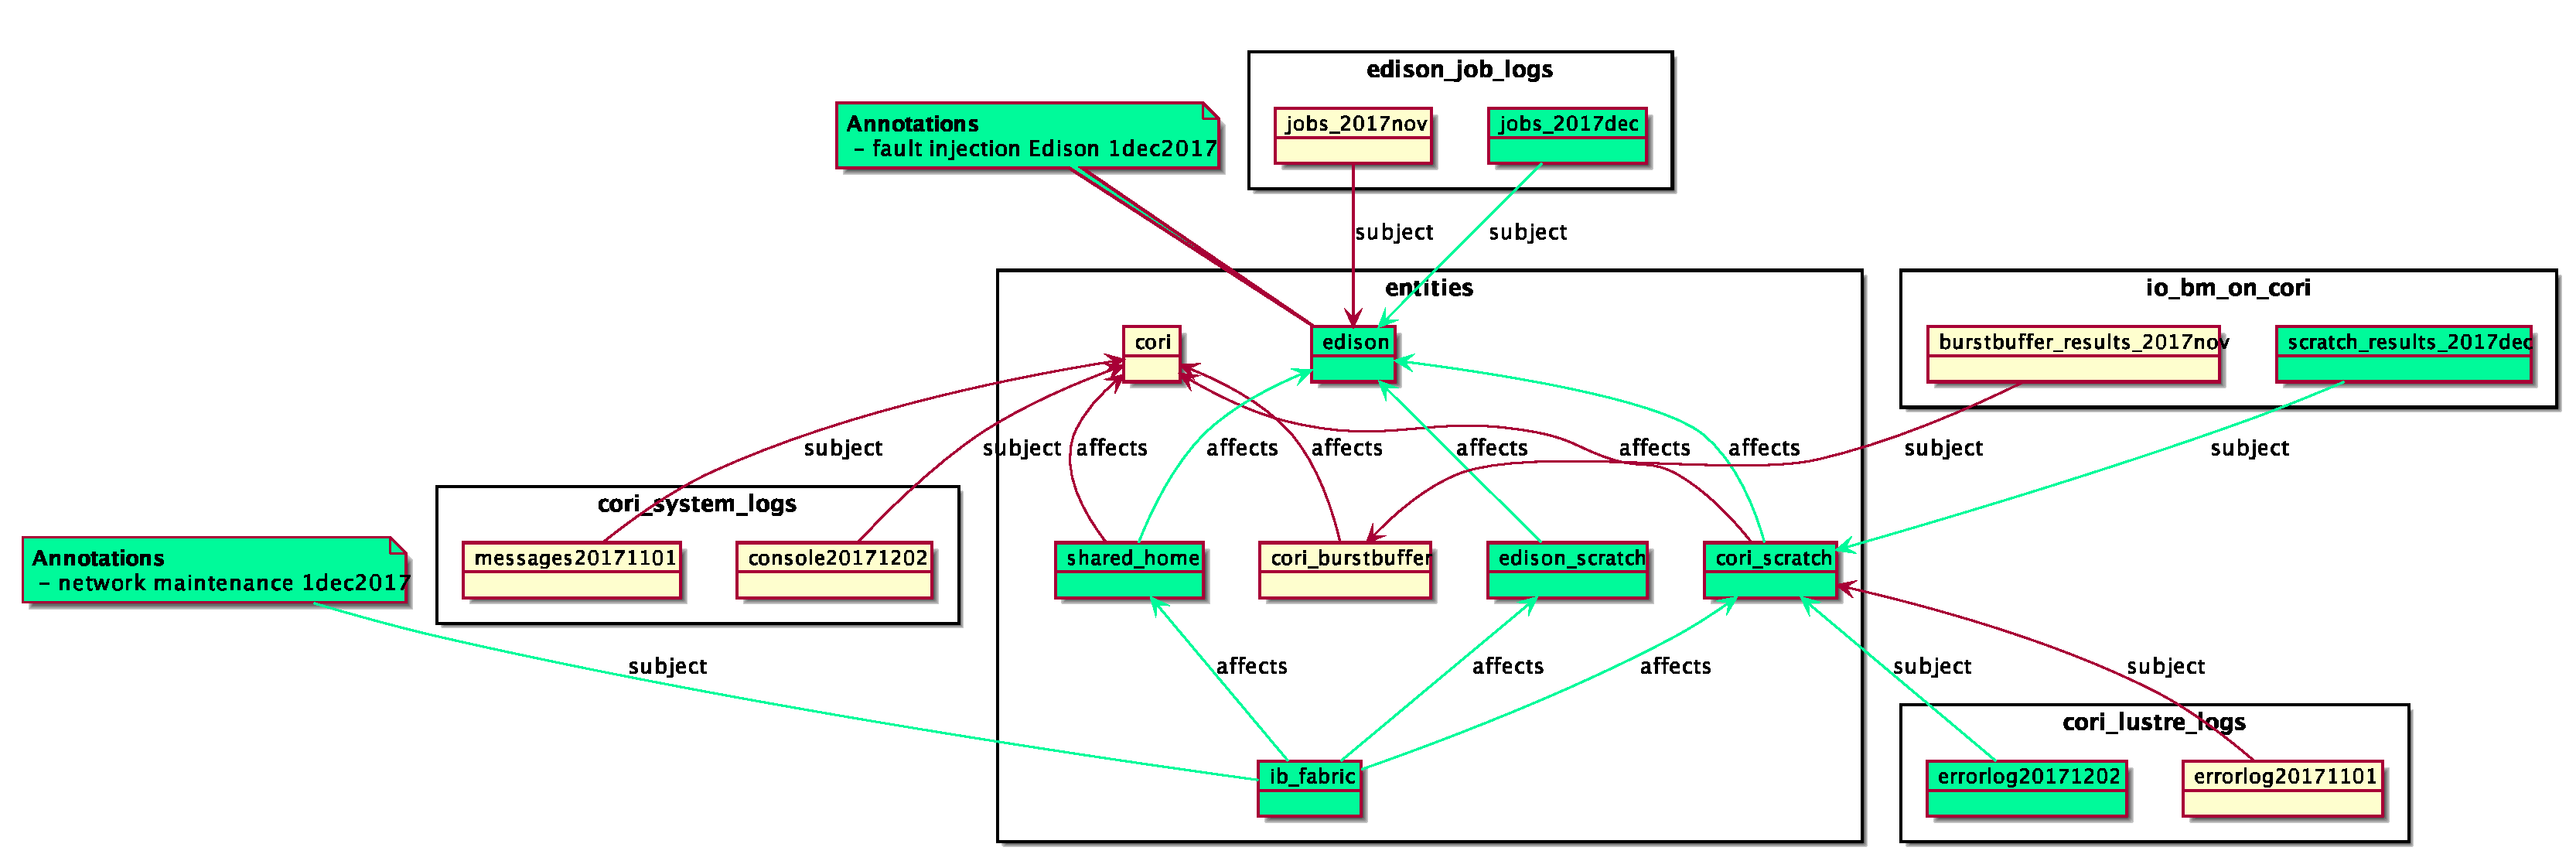
\includegraphics[width=0.9\textwidth]{datasets-example}
%  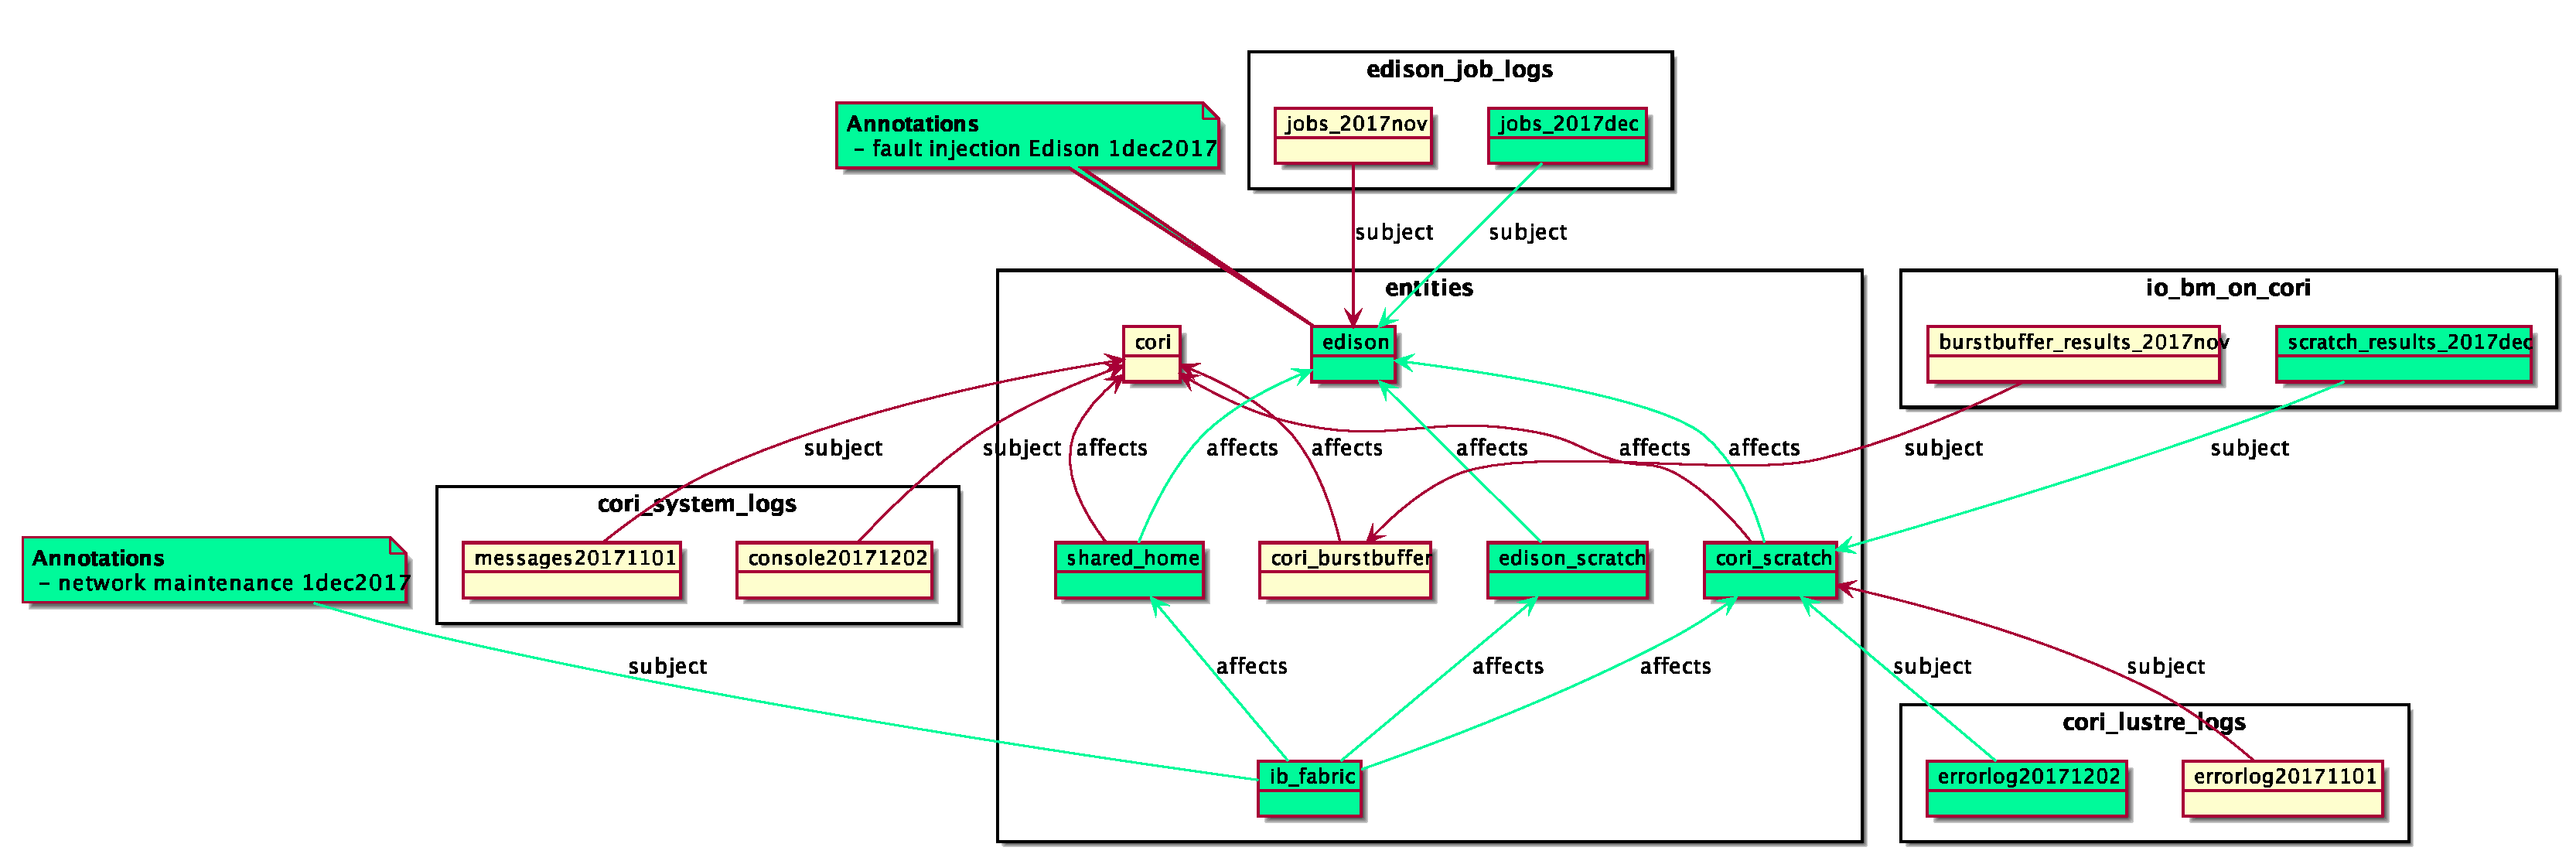
\includegraphics[height=3cm]{datasets-example}
  \caption{Querying a distributed graph from multiple
contributors for logs and annotations related to a particular system at a
particular time.}
\end{figure*}

\section{Contributions of this paper}
We present a solution for annotating log data with human-made observations, and
for publishing and discovering annotations and log data without imposing an
unsustainable burden of effort on either those collecting data or those
analyzing it.

\begin{itemize}
\item We present a mechanism to publish descriptions of collected data
% so as to be
wherby data is easily discoverable with existing linked-data tools, without
reliance on existing knowledge of who is collecting or using which data.
%and requires no heroic effort on the part of either.
By requiring minimal effort we enable a sustainable ecosystem of data collection
and analysis.

\item We present a schema for annotations in which human (or machine-generated)
observations can be published and linked to log data. The schema supports
observations associated with both an imprecise timespan and with specific log
entries; and allows disparate observations of the same subject to be combined. A
set of annotations is a dataset in its own right and can be published and
discovered in the same way.

\item We present tools to help generate, publish, and discover these annotations.
This will enable annotators, data collectors, and researchers to perform typical tasks
and queries without the need to learn the underlying technologies (i.e.,
SQL, RDF and SPARQL).

\item We present case studies demonstrating the use and benefits these on a
a large (Cori) Cray system and a small testbed at different sites.
These tools can support other Cray
sites in sharing and using annotated datasets to better understand and mitigate
faults
%propagation
in Cray systems.
\end{itemize}

\section{Annotation}
Annotations can enable domain experts to provide meaningful information 
(e.g., event descriptions, log entry meanings) required for analysts, without 
domain knowledge, to gain useful insights from otherwise meaningless data.
%Annotations allow those with domain knowledge to describe an event and identify
%relevant log entries so as to be meaningful to analysts without that domain
%knowledge. 
We present an annotation schema allowing human-described events to
be accessed via the same interface as log entries, thus allowing observations
to be overlaid on log entries for investigation of events of interest.

Our schema is a set of SQL tables whose entries describe an event with regards
to timespan, state of the system before and after, and related events. Entries
can be mapped to record-identifiers for specific log types. This enables 
description of events by both approximate timespan and 
%also to call out
specific relevant log entries.

The schema includes provenance information and is designed to support merging of
annotation entries from multiple sources.

\section{Discovery}
The integration of diverse but related information is a motivating case for
linked data and semantic web technologies. It also describes the challenge
faced by researchers investigating resiliency on Cray and other large systems.
Therefore we have based our discovery mechanism on established linked-data
technologies.

We extend the W3C DCAT (Data Catalog) vocabulary to specifically cover log-like
data, including access and format details, and use the ADMS (Asset
Description) and FOAF (Friend-of-a-Friend) vocabularies to describe the subjects
and publishers of monitoring data.

Datasets and catalogs form a queryable, distributed graph of URIs. A site can
publish a catalog of local data with links to a few other catalogs. Local
staff can add links in their local catalog to their own data which then
becomes part of the global graph. Figure 1 illustrates how data added from
disparate sources forms a single graph that can be queried to find all logs
that might have contributed to an event on a specific system (Edison) at a
particular time.

Our annotation schema allows human-made observations to integrate into this
graph, providing both a data point and a starting point for new queries

A key point is that the graph is comprised only of metadata. The log data
itself typically has constraints around security, privacy, or sheer volume.
Data is collected primarily for a specific internal use and the effort required
to clean and publish it for ``the greater good" is generally enough to prevent it
from being published. By asking collectors to publish only metadata we reduce
the publishing effort to a sustainable level.

\section{Putting it all together}
The learning curve for using the underlying SQL and linked data technologies
itself presents an obstacle to publishing and using log data, but most use
cases for publishers, annotators and analysts are based on only a few queries.
To mitigate this obstacle we provide tools that guide users through common
tasks without requiring direct use of SQL or SPARQL. This does not preclude
direct use of the underlying technology by those comfortable with it.

Finally, we present case studies on systems at different sites illustrating the mechanism,
benefit, and general applicability of the tools and schema presented here. Cases include:

\paragraph{User investigation of system events impacting job performance} Application
performance can be impacted by events which are apparent in log data but not exposed to 
users or not apparent to someone without appropriate domain knowledge to interpret the
log data. Our framework enables investigation by users or support staff by exposing 
expert translations of significant occurrences without necessarily exposing logs beyond
their normal security and privacy domain. In addition, the framework enables users to
identify and specify to support staff relevant slices of logs they cannot directly 
access, reducing the effort required by support staff to aid in such questions.

In this example, we show how a user can investigate underlying reasons for and
occurrences of performance variation issues by integrated access of expert annotations 
of CPU throttling events, link degrades, and memory errors which occur in disparate 
Cray logs in conjunction with historic job data.

\paragraph{Administrator event investigation}
The historical state of the system includes not only events captured by the logs, but
human-invoked actions as well, such as DIMM replacement, software upgrades, and cable reseating.
Our annotation system enables labeling and search of both human-defined and system-defined events
in a consistent way, and the return of such events in a format suitable for plotting or additional analysis.

This example shows how the investigation of component faults and resolution can be facilitated by our
framework. Sequences of failures followed by manual resolution action are easily discoverable and visualized
in a timeline. The easy determination of the time between problem onset and resolution is useful for
reporting of the system impact of particular component problems. Finally, long term analysis is used to
detect components (e.g., nodes) which indicate more faults over time, regardless of replacement, which can indicate that
the root cause of problems is environmental (e.g., temperature) rather than component-based.

A related example demonstrates characterization of the impacts of
events which are resolved by the system itself: network failure events which should be resolved by the automatic recalculation
of network routes. Using our framework on production and
fault injection data, we show how the timescales of impact are easily discovered, as well as the discovery
of events for which successful rerouting did not occur. Identification of these occurrences also then facilitates
direction to regions of the logs for more in-depth analysis as to the circumstances of the failure.










% conference papers do not normally have an appendix


% trigger a \newpage just before the given reference
% number - used to balance the columns on the last page
% adjust value as needed - may need to be readjusted if
% the document is modified later
%\IEEEtriggeratref{8}
% The "triggered" command can be changed if desired:
%\IEEEtriggercmd{\enlargethispage{-5in}}

% references section

% can use a bibliography generated by BibTeX as a .bbl file
% BibTeX documentation can be easily obtained at:
% http://www.ctan.org/tex-archive/biblio/bibtex/contrib/doc/
% The IEEEtran BibTeX style support page is at:
% http://www.michaelshell.org/tex/ieeetran/bibtex/

%%%% YOU CAN ADD IN ADDITIONAL BIB FILES BELOW %%%

%\bibliographystyle{IEEEtran}
%\bibliography{IEEEabrv,./test}
% argument is your BibTeX string definitions and bibliography database(s)
%\bibliography{IEEEabrv,../bib/paper}
%
% <OR> manually copy in the resultant .bbl file
% set second argument of \begin to the number of references
% (used to reserve space for the reference number labels box)
%\begin{thebibliography}{1}
%\end{thebibliography}




% that's all folks
\end{document}
